\documentclass {article}
\usepackage {graphicx}
\usepackage [margin=1in]{geometry} %border Margins
\usepackage {hyperref}
\usepackage [table,xcdraw]{xcolor}
\usepackage {booktabs} %Allow tables to be created well
\usepackage {titlesec} %Allow subsubsubsection
\usepackage {float} % To make table appear where you place its code
\usepackage {mathpazo}
\usepackage {appendix}
\usepackage [style=apa, backend=biber]{biblatex} % To write references in APA 7 format
\linespread{1.6}
\usepackage {titlesec}
\titleformat{\section}{\Huge\bfseries}{\thesection}{1em}{}
\titleformat{\subsection}{\LARGE\bfseries}{\thesubsection}{1em}{}
\titleformat{\subsubsection}{\Large\bfseries}{\thesubsubsection}{1em}{}
\fontsize{12pt}{16pt}\selectfont
\renewcommand{\normalsize}{\fontsize{12}{16}\selectfont}


% \renewcommand{\subsection}{\fontsize{12pt}{16pt}\selectfont}
% \titleformat{\subsection}{\Large\bfseries}{\thesection}{1em}{}

\addbibresource{citation.bib}

\makeatletter
\def\subsubsubsection{\@startsection{subsubsubsection}{4}{\z@}%
{-3.25ex\@plus -1ex \@minus -.2ex}%
{1.5ex \@plus .2ex}%
{\normalfont\normalsize\bfseries}}
\makeatother

% \bibliographystyle{apa7}
\begin{document}

\title{\textbf{TOPIC:  DIET AND NUTRITION MANAGEMENT SYSTEM} }
\author{Sensy}
\date{October, 2022}
\begin{center}

\textbf{\Huge{MAKERERE}} \includegraphics[width=70px]{Images/muk_logo.png} \textbf{\Huge{UNIVERSITY}}


\begin{center}
\large{\textbf{COLLEGE OF COMPUTING AND INFORMATION SCIENCES\\ SCHOOL OF COMPUTING AND INFORMATICS TECHNOLOGY}}

\end{center}

\hrule

\vspace{20px} 


\vspace{-9pt} 

\begin{center}
\textbf{Department of Information Systems}\\
\textbf{School of Computing and Informatics Technology}
\\ BIST:(Systems Development)
\end{center}
\vspace{20px} 

{\LARGE TOPIC:  DIET AND NUTRITION MANAGEMENT SYSTEM}\
\vspace{5px} 

\begin{center}
\textbf{A Proposal submitted to the College of Computing and Information Sciences in Partial fulfillment of the Requirements for the Award of a Degree of Bachelor of Information Systems and Technology of Makerere University.}
\end{center}

% \vspace{200pt} 
\vspace{3pt} 
\textbf{Supervisor:} Mr. Bitwire Albert George \\
 bitwire.albert@gmail.com \\ +256 773-095119 \\
\vspace{25pt}
\textbf{
Sign:...............................\hspace{40pt}Date:............................... \\
}
\vspace{25pt}


% \textbf{Option:} Systems Development
\end{center}
\newpage

\begin{center}
PRESENTED BY:
\end{center}
\vspace{20pt}


\begin{table}[h]
% \centering

\LARGE
\setlength{\tabcolsep}{6pt}%sets the horizontal (column) spacing
\renewcommand{\arraystretch}{2} %sets the vertical (row) spacing
\resizebox{\textwidth}{!}
{
\begin{tabular}{|c|c|c|c|c|}
\hline
\textbf{NAME} & \textbf{STUDENT NO} & \textbf{REG NO} & \textbf{E-MAIL} & \textbf{CONTACT}\\
\hline
MUHUMUZA VICTOR IAN & 2000703524 & 20/U/3524/PS & viktamuhumuza@gmail.com & 0761-656330\\
\hline
WAKOKO SIMON PETER & 2000703512 & 20/U/3512/PS & peterwakoko@gmail.com  & 0775-362626\\
\hline
KIKOMEKO PETER GRACE & 2000703578 & 20/U/3578/PS & gracekikomeko@gmail.com & 0775-939664\\
\hline
NAMBOOZE RACHAEL & 2000707994 & 20/U/7994/EVE & racheal.nambooze@students.mak.ac.ug & 0755-868603\\
\hline
ONEN SAM SENSY & 2000703502 & 20/U/3502/PS & sensyonen@gmail.com & 0782-150448\\
\hline
\end{tabular}
}
\end{table}

\newpage
%Table of content
\tableofcontents
\newpage
%List of tables
\listoftables
\newpage
%List of figures
\listoffigures
\newpage

\section{Introduction}
\label{Introducion}

\subsection{Introduction}
Information systems are concerned with data capture, storage, analysis, and retrieval. These are vital to assist decision-making in a short time frame, potentially allowing decisions to be made and practices to be action-ed in real time.  In the context of diet and nutrition management, nutritional health systems allow for accurate and efficient analysis of food ingredients as well as patient nutrient intake which assists in ensuring that selected food combinations offer the desired nutrients for a particular meal or diet(\citeauthor{DFM}, \citeyear{DFM}). 


\subsection{Background}
\label{Background}
\noindent Dietary deficiency is more accountable for the overall death toll on the global scale than other factors such as tobacco, high blood pressure, or any other health risk, as indicated in the new scientific study. “Poor diet is an equal opportunity killer,” (\citeauthor{ihme2019new}, \citeyear{ihme2019new}). Low levels of healthy food consumption, such as whole grains, in contrast to too many unhealthy foods, including sweetened beverages, account for one in every five deaths globally, “We are what we eat and risks affect people across a range of demographics, including age, gender, and economic status,” (\citeauthor{ihme2019new}, \citeyear{ihme2019new}).\\

\noindent Poor diets were behind the 10.9 million deaths, or 22\% of all deaths among adults in 2017, with cardiovascular disease (CVD) as the foremost cause, trailed by cancers and diabetes. They also resulted in 255 million disability-adjusted life years (DALYs), equaling the sum of years lost and years lived with disability. Poor diet statistically represents 16\% of all DALYs among adults globally. The findings of the study indicate that while the impact of individual dietary factors varies across countries, three dietary factors – low intake of whole grains, as well as fruits, and high consumption of sodium – accounted for more than 50\% of diet-related deaths and 66\% of DALYs. The other 50\% of death and 34\% of DALYs were tied to high consumption of red meat, processed meats, sugar-sweetened beverages, and trans fatty acids among other foods. There is an urgent and compelling need for changes in the various sectors of the food production cycle, such as growing, processing, packaging, and marketing (\citeauthor{ihme2019new}, \citeyear{ihme2019new}).\\

\noindent Uganda has shown limited progress towards achieving the diet-related non-communicable disease (NCD) targets. Furthermore, it has shown no progress towards achieving the target for obesity, with an estimated 10.4\% of adult (aged 18 years and over) women and 2.3\% of adult men living with obesity. Uganda's obesity prevalence is lower than the regional average of 20.7\% for women and 9.2\% for men. At the same time, diabetes is estimated to affect 5.6\% of adult women and 5.6\% of adult men (\citeauthor{globalnutritionreportn.d.}, \citeyear{globalnutritionreportn.d.}). The motivation for feeding should not only be to stop hunger, but also to increase the general awareness of the nutritional value of the food ingested.

\subsection{Problem statement}
\noindent Improper diet and nutrition are caused by inconsistent intake of healthy foods. Other causes include improper meal timings, under or overeating, not having enough healthy foods, and nutritional ignorance. Experts have revealed that only 10\% of children below the age of five years are eating recommended healthy foods and this includes frequenting eating nutritious meals and eating on time. This has left the majority 90\% eating non-nutritious foods which has resulted in increasing numbers of childhood malnutrition and obesity (\citeauthor{tumwine2022only}, \citeyear{tumwine2022only}). “People are eating a lot of unhealthy foods that do not contribute to the manufacturing of blood in the body which has made them sicker.”(\citeauthor{tumwine2022only}, \citeyear{tumwine2022only}). We therefore intend to contain this problem by developing a diet and nutrition management system which will guide the targeted populace categories majorly students to maintain a healthy selection of well-balanced meals daily.

\subsection{Objectives}
\subsubsection{General Objectives}

\noindent To develop a diet and nutrition management system that will provide students with timely suggestions on the food they should consume to remain healthy. 

\subsubsection{Specific Objectives}

\begin{enumerate}
    \item To identify the requirements for a Diet and Nutrition Management System in order to understand what the would-be users of the system would want.
    \item To design a model for the system.
    \item To implement the system.
    \item To test and validate the system. 
\end{enumerate}


\subsection{Justification.}
\noindent Improper diet and nutrition is a constant challenge to many students which adversely exposes them to risks like obesity, digestive problems, and chronic illnesses. From the effects, our system intends to; \\

\noindent Increase awareness on the dire consequences of improper diet and nutrition. Proper diet and nutrition is essential to maintaining good health, yet many people are not aware of the serious consequences that can result from a poor diet. To address this, it is important to raise awareness and educate people on the importance of a balanced diet and the potential health risks associated with poor nutrition.\\

\noindent Provide a practical means to improve feeding patterns daily. One of the most effective ways to improve dietary patterns is to provide a practical and user-friendly means for people to monitor and track their daily food intake. This can include tools such as nutrition tracking apps, meal planning guides, or online resources that provide recipe ideas and tips for making healthy food choices. \\

\noindent Customize a system to the needs of Students Population. The dietary needs of students are unique and differ from other population groups. It is important to customize a diet and nutrition management system to meet the specific needs of this population group. This can include taking into account the limited time and resources that students often have, as well as the specific nutritional requirements of growing bodies.
\subsection{Scope}
\noindent Our research will be focused on locally grown foods in Uganda that consist of a balanced diet and specific chronic illnesses like Diabetes, obesity, pressure and cancer. We will major at Makerere University. We intend to sample several students from colleges such as CEDAT, COCIS, and CHUSS to know the foods they regularly eat.

\subsection{Significance}

\noindent The system that we aim to build will help University students select the best food combinations within the appropriate time through timely reminders and food suggestions, while additionally providing Nutrition Literature.

\subsection{Conclusion}
\noindent In conclusion, information systems play a crucial role in diet and nutrition management by providing the tools for data capture, storage, analysis, and retrieval. These capabilities allow for efficient and accurate analysis of food ingredients and patient nutrient intake, which in turn assist in ensuring that selected food combinations provide the desired nutrients for a particular meal or diet. By providing real-time decision-making capabilities, these systems have the potential to improve the effectiveness of dietary and nutrition management practices.

%%-------------------------------------------------------------------------------
%% 2.0 Literature review
%%-------------------------------------------------------------------------------
\newpage
\section{Literature Review}

\subsection{Introduction}
\noindent According to Wikipedia (\citeyear{wikipedia2019dietary}), dietary management simply means providing nutritional options for individuals and groups with diet concerns through the supervision of food services. Information systems have made it easier for accurate and efficient nutritional analysis of feeding habits and patterns.\\

\noindent This section focuses on the exploration of different solutions developed by researchers to alleviate the problem of poor eating habits among University students. We reviewed similar systems regarding the problems faced by students when they skip meals or even fail to eat at the right time. The solution we aim to provide for this problem is to develop a diet and nutrition management system that will provide students with timely reminders, food suggestions, and nutrition literature.\\

\noindent We realized that so much research has been done by researchers from the field of nutrition science where a person is trained to provide information regarding the types and quantities of food the people eat. This field draws information from other areas such as biology, chemistry, and social sciences (\citeauthor{sriram2020hire}, \citeyear{sriram2020hire}).\\

\noindent The review is comprised of works that have been done to find the solution to the problem and we were able to sample various systems. We singled out systems that were closely related to our research problem and we noted the strengths and weaknesses of the solutions. By studying these systems, we were able to find the deficiency in the solutions regarding our problem and stated ways in which the solutions can be tailored to satisfy our target group. The features of the reviewed systems are compared with those of the proposed system in Table 1.\\

\subsection{Existing Systems}

\subsubsection{MantraCare}

\noindent MantraCare, (\citetitle{mantracare}, n.d), is a Ugandan web-based application that offers a range of tools and resources for individuals looking to improve their health and manage their diet. Its services include consultation services with dieticians on belly fat reduction and weight loss dieting plans, exercises, and foods and may more.\\

\noindent \textbf{Strength of the System: \\}
\noindent MantraCare offers personalized meal planning that takes into account individual dietary restrictions and goals. This service is designed to meet the unique needs of every user, ensuring that they receive a meal plan that is tailored to their specific dietary restrictions and goals. This can include accommodating with allergies, medical conditions, or weight loss goals.\\

\noindent Users can also take advantage of comprehensive nutrition tracking. With MantraCare, users can track their daily intake of nutrients including calories, carbohydrates, protein and fats, giving them a clear picture of their dietary intake. This allows them to make informed decisions about their diet and make changes to improve their nutrition.\\

\noindent In addition, MantraCare provides access to a variety of resources such as recipe ideas, nutrition articles, and exercise guides. These resources are designed to help users make informed decisions about their diet and lifestyle. They can be used as a reference for meal planning or for inspiration when creating new recipes.\\

\noindent Additionally, MantraCare's community of users and professionals can provide support and guidance on nutrition and diet management. Users can connect with other users and professionals to share advice, tips and support. This can be especially helpful for those who are new to diet and nutrition management and need guidance on how to get started.\\


\noindent \textbf{Weaknesses of the System: \\}
\noindent Cost: MantraCare requires a subscription fee, which may be a barrier for some users. This can limit its accessibility to individuals who may not be able to afford the subscription fee. It may not be a good fit for those on a tight budget.\\

\noindent It does not offer food suggestions. This may make it difficult for users to know what to eat, especially if they are not familiar with healthy food options. This can make it difficult for users to stick to their diet plan. \\

\noindent Limited customization: While MantraCare offers personalized meal planning, the options may be limited for those with specific dietary needs or preferences. This can make it difficult for users with food allergies or sensitivities to find suitable options. This may limit the effectiveness of the meal planning for some users.\\

\noindent Lack of in-person support: As an online platform, MantraCare does not offer in-person support or consultation with nutrition professionals. This can make it difficult for users to get the support they need to make changes to their diet and lifestyle. This can make it difficult for some users to achieve their health goals.
\subsubsection{LifeSum}
% LifeSum is a fitness app that lets you decide what a healthy lifestyle means to you. It has plenty of recommendations and suggestions, but they are always pointing toward the goal you want.

Lifesum (\citetitle{lifesum}, n.d) is a digital health and wellness platform that aims to help users improve their overall health through personalized nutrition and exercise recommendations that always pointing toward the goal you want. It offers a range of features, including a food diary, macro tracking, and fitness tracking, as well as personalized meal plans and recipe suggestions.\\

\noindent \textbf{It has several features which include: \\}
\noindent Simple tracking of meals (including barcode scanning), exercises, habits, weight, and body measurements. This allows users to easily track their progress and make adjustments to their diet and exercise routine.\\

\noindent A wide range of diets to choose from, including Ketogenic Diet. This provides users with the flexibility to choose a diet plan that best suits their needs and goals.\\

\noindent Favorites - save your favorite food, exercises, meals, and recipes. This makes it easy for users to quickly access their preferred meals and exercises.\\

\noindent Meal plans - 1 to 3 weeks of scheduled, easy-to-cook meals. This helps users to plan and prepare their meals in advance, making it easier to stick to their diet.\\

\noindent Support for macros and net carbs. This provides users with detailed nutritional information, making it easier to track their macronutrient intake.\\

\noindent Detailed nutritional information. This helps users to make informed decisions about the food they eat and ensure they are getting the nutrients they need.\\

\noindent Food, meal, and day ratings. This allows users to rate their meals and track their progress over time.\\

\noindent Weekly life score - what’s gone well and how you can improve. This helps users to reflect on their progress and identify areas where they can make improvements.\\

\noindent Hundreds of healthy and tasty recipes. This provides users with a wide range of meal options to choose from.\\

\noindent Integrates with Apple Health, Google Fit, Samsung Health, Apple Watch, RunKeeper, Fitbit, Withings, Samsung wearable devices, Wear OS and Google Assistant. This allows users to seamlessly track their progress and access their data across multiple devices.\\

\noindent \textbf{Strengths of the System:\\}
\noindent The ability to integrate with different technologies for example Google Fit, and Apple Watch among others. This allows users to seamlessly track their progress and access their data across multiple devices.\\

\noindent Wide range of features for comprehensive health and wellness tracking. This provides users with the ability to track various aspects of their health and wellness, including their meals, exercise, and body measurements.\\

\noindent Personalized meal plans and recipe suggestions. This helps users to plan and prepare their meals in advance, making it easier to stick to their diet and achieve their health goals.\\

\noindent Integration with popular fitness tracking devices and apps. This allows users to easily track their progress and make adjustments to their diet and exercise routine.\\

\noindent Available in multiple languages. This allows users to access the app in their preferred language, making it more user-friendly and accessible.\\

\noindent \textbf{Weaknesses of the System:\\}
\noindent Some users have reported difficulties with the food diary and tracking accuracy. This may make it harder for users to accurately track their food intake and make adjustments to their diet.\\

\noindent Premium subscription required for access to certain features. This may act as a barrier for some users and limit their access to the full range of features offered by the app.\\

\noindent Limited availability of certain features (e.g. personalized meal plans) in certain countries. This may limit the app's usefulness for users in certain regions, making it less accessible to them.\\


\subsubsection{My Plate Calorie Counter}

\noindent My Plate Calorie Counter (\citetitle{myplate}, n.d) is a popular nutrition and diet management solution developed by the U.S. Department of Agriculture (USDA). It offers a range of features designed to help users make healthier food choices and track their daily nutrient intake. They use the world’s largest food database to provide you with calorie counts, nutritional information, and serving sizes for lots of foods. You can also access an 8-week meal plan and recipe suggestions.\\

\noindent \textbf{Strengths of the system:\\}
\noindent Provides a comprehensive database of over 8,000 foods, including common brand names and restaurant meals. This allows users to easily track their food intake and make informed decisions about the food they eat.\\

\noindent Offers personalized daily calorie and nutrient recommendations based on the user’s age, gender, weight, height, and physical activity level. This helps users to ensure they are getting the right amount of nutrients for their body type and lifestyle.\\

\noindent Allows users to track their daily intake of macro-nutrients (protein, carbohydrates, and fat) and micro-nutrients (vitamins and minerals). This provides users with detailed nutritional information, making it easier to track their macronutrient intake.\\

\noindent Integrates with popular fitness apps, such as MyFitnessPal and Fitbit, to provide a more comprehensive view of the user’s overall health and wellness. This allows users to seamlessly track their progress and access their data across multiple devices.\\

\noindent Offers educational resources and tips on healthy eating and weight loss. This provides users with the knowledge they need to make informed decisions about their diet and lifestyle.\\

\noindent \textbf{Weaknesses of the system: \\}
\noindent Most of the suggested foods such as Southwestern Pancakes, chocolate Almond protein cocoa, and many others are alien to our target group, which are the university students in Uganda. This makes it difficult for them to follow the suggested meal plans.\\

\noindent If you want to get the most out of the app such as your highest caloric foods, daily goals, and personal progress, you are required to subscribe to the app which 1 month costs \$9.99 (approximately Ugx 38,000/=) . This cost would be a barrier for most of the students.\\

\noindent This option would not work for our target group because the suggested foods are hard to find in Uganda and if they are available, they would be so expensive for the students.\\

\noindent Some users have reported issues with the app’s tracking feature, including difficulty inputting custom foods and incorrect calorie counts. This can make it difficult for users to accurately track their food intake and make adjustments to their diet.\\

\noindent Some users have reported issues with the accuracy of the nutrient information provided in the database. This can lead to confusion and mistrust among users, making it difficult for them to make informed decisions about their diet.\\

\noindent The app is only available for iOS and Android devices, which may exclude users who do not have access to these types of devices. This limits the app's accessibility and could make it less useful for some users.\\

\subsubsection{The Diet Planner Application}

\noindent The Diet Planner Application (\citetitle{dietplannerapp}, n.d), is a dietary management system that is equipped with features such as 10,000 ready meals, 270 allergens, patients' medical report capability, meal plans, personalized patient menus, nutritional interviews, kitchen and home measures, and a search engine for dishes and products, etc. To save patients' time, specialists create balanced meals that can be enjoyed without restrictions. It will allow for the preparation of nutrition plans for patients faster than ever. It enables the instant generation of fully personalized menus by a wide range of calorie goals, preferences, and dietary restrictions.\\

\noindent \textbf{Strengths of the System:\\}
\noindent It can generate a health report for the user, which allows them to track their progress over time and make adjustments to their diet and lifestyle as needed. This can be a valuable tool for users who are working to improve their overall health and wellness.\\

\noindent It has a search engine for dishes and products, which can make it easier for users to find and track the foods they are eating. This can be especially useful for users who are trying to stick to a specific diet or who have food allergies or sensitivities. The search engine allows users to quickly and easily find the information they need to make informed decisions about their food choices.\\

\noindent \textbf{Weaknesses of the System: \\}
\noindent It does not have timely reminders, which can make it difficult for users to stay on track with their diet and nutrition goals. Without reminders, users may forget to track their meals or miss important nutrient intake.\\

\noindent It also does not have a BMI (Body Mass Index) calculator, which is an important tool for users to monitor their weight and overall health. A BMI calculator can help users determine if they are at a healthy weight and make adjustments to their diet and exercise routine as needed. Without this feature, users may have a harder time understanding their body composition and making informed decisions about their health.\\

\subsubsection{Nutrition and Diet Management Solutions by Nutritics}

\noindent Nutrition and Diet Management Solutions(\citetitle{nutritics}, n.d) is a software platform that provides a range of tools and resources for professionals in the field of nutrition and dietetics. The platform includes features such as a nutritional assessment tool, a meal planning module, and a recipe database, as well as educational resources such as articles and webinars. It allows multiple profile details designated as clients to be entered. Each profile is then analyzed and then, a tailored meal plan is suggested according to the profile that has been entered.\\

\noindent \textbf{Strengths of the system: }\\
\noindent The Nutrition and Diet Management Solutions system offered by Nutritics includes a variety of support options for its users, including the use of webinars as a means of providing information and assistance. In addition to webinars, the system may also offer other forms of support such as email or phone support, online resources or tutorials, and in-person support through local events or workshops. This comprehensive support network helps users to make the most of the system and achieve their nutrition and diet goals.\\

\noindent It provides the user with a variety of options for meals, allowing them to choose different alternatives to fit their dietary needs and preferences.\\

\noindent It has multiple categories of users that it focuses on, including individuals looking to improve their personal nutrition and healthcare professionals looking to manage their patients’ dietary needs.\\

\noindent It allows the user to add new food items and their corresponding nutritional information to the system, which helps in keeping track of the nutritional intake of individuals and making informed dietary decisions.\\

\noindent Wide range of features: Nutritics offers a range of features including meal planning, recipe analysis, and nutritional assessment tools, making it a comprehensive resource for nutrition professionals and individuals.\\

\noindent User-friendly interface: The platform has a user-friendly interface that is easy to navigate, making it accessible to users of all levels of experience.\\

\noindent Customization options: Nutritics allows users to customize their experience by setting specific goals, dietary preferences, and other parameters.\\

\noindent Accurate and reliable: Nutritics uses reliable sources and evidence-based guidelines to provide accurate and up-to-date information on nutrition and diet management.\\

\noindent \textbf{Weaknesses of the System: \\}
\noindent The platform may not be accessible to all users due to the cost of subscription. This can be a barrier for some individuals who may not have the financial means to subscribe.\\

\noindent The application is customized for desktops only. This means that users will need access to a computer in order to use the platform.\\

\noindent The application is customized for organizations or hospitals to manage multiple clients/patients. This makes it a useful tool for healthcare professionals who are looking to track the nutrition of multiple patients.\\

\noindent The system is based on expensive meals that may not be affordable. This can be a challenge for individuals who are on a budget and may not be able to afford the recommended meals.\\

\noindent Lack of personalization: While Nutritics does offer customization options, it may not be able to provide the same level of personalization as a one-on-one consultation with a nutrition professional. This means that users may not be getting the same level of personalized advice and support as they would with a professional consultation.\\

\subsubsection{Noom}
Noom(\citetitle{noon}, n.d) is a nutrition and diet management solution that utilizes a combination of artificial intelligence and human coaching to help users make healthier lifestyle choices. One strength of Noom is its personalized approach, as the program tailors its recommendations and goals to the individual user. Noom also offers a wide range of resources and support tools, including educational articles, tracking tools, and the option for one-on-one coaching sessions\\

\noindent \textbf{Strengths of the system: \\}
\noindent Noom provides a comprehensive weight loss program that includes personalized meal plans, exercise tracking, and goal setting. This allows users to tailor their program to their specific needs and goals.\\

\noindent The program also offers one-on-one coaching from certified health coaches, providing support and accountability for users. This means that users have access to professional guidance and support throughout their weight loss journey.\\

\noindent Noom’s focus on creating sustainable lifestyle changes rather than quick fixes is a key strength, as it helps users maintain their weight loss over the long term. This approach is more effective in the long run and helps users to create healthy habits that will last a lifetime.\\

\noindent The program is backed by scientific research and has been shown to be effective in multiple clinical studies. This gives users confidence in the program and its effectiveness.\\

\noindent Noom offers a range of resources and tools for users, including a food diary, articles and tips on healthy living, and a supportive online community. This provides users with a comprehensive program that includes not just weight loss but also education and support.\\

\noindent It is available both on mobile and desktops. This means that users can access the program from anywhere, at any time, making it convenient and easy to use.\\

\noindent \textbf{Weaknesses of the system: \\}
\noindent It has so many questions that take almost an hour to be answered. This can be time-consuming and may deter some users from signing up.\\

\noindent Some users may find the cost of Noom’s program to be a barrier, as it is more expensive than some other weight loss programs. This can be a challenge for those who are on a tight budget and are looking for more affordable options.\\

\noindent The program requires a significant time commitment, as users are expected to track their meals, exercise, and progress regularly. This may not be feasible for individuals who have busy schedules or limited time.\\

\noindent Some users may find the emphasis on tracking and goal setting to be too structured, and may prefer a more flexible approach. This may not be suitable for those who are looking for a more relaxed and less restrictive program.\\

\noindent Noom’s program may not be suitable for those with certain medical conditions or food allergies, as it does not offer specialized meal plans for these groups. This can be a challenge for those with specific dietary needs.\\

\noindent The program may not be as effective for those who are severely overweight or obese, as it is primarily focused on helping people lose smaller amounts of weight. This may not be the best option for those who have a lot of weight to lose.\\

\noindent It is not accessible in terms of affordability to people like students. This can be a barrier for those who are on a tight budget and are looking for more affordable options.\\

\subsection{Proposed System}
\noindent As a group, we shall develop a web-based application that will require university students to register possibly with their name and email addresses that will be used to send notifications to eat food cost-effectively. After this, they will be able to receive timely reminders on the minimum amount and type of food they should consume to successfully fulfill their daily tasks. This will include a mix of foods such as Matooke, Rice, and Sweet potatoes and drinks such as water and a cup of tea. It will also include general knowledge on how they can maintain a healthy and functioning body such as drinking lots of water, exercising regularly, and avoiding harmful consumption of alcohol, and drugs among others.
This will provide a more customized and cost-effective feeding way for university students to allow them to focus on their studies as they also take care of their health.

\begin{table}[H]
\centering
\caption{Comparison Of the Systems}
\label{tab:comparison-of-systems}
%--------------------------------
% Spacin Added By Victor
\setlength{\tabcolsep}{6pt}%sets the horizontal (column) spacing
\renewcommand{\arraystretch}{1.5} %sets the vertical (row) spacing
%--------------------------------
\resizebox{\columnwidth}{!}{%
\begin{tabular}{|l|l|l|l|l|l|l|l|}

\hline
\textbf{System Features}  & \textbf{MantraCare} & \textbf{\begin{tabular}[c]{@{}l@{}}Nutrition and Diet \\ Management Solutions\\  By Nutritics\end{tabular}} & \textbf{Noom} & \textbf{\begin{tabular}[c]{@{}l@{}}Diet \\ Planner\end{tabular}} & \textbf{\begin{tabular}[c]{@{}l@{}}My Plate \\ Calories\end{tabular}} & \textbf{Life Sum} & \textbf{\begin{tabular}[c]{@{}l@{}}Proposed \\ System\end{tabular}} \\ \hline
BMI Calculator &  & \textbf{YES} & \textbf{YES} &  & \textbf{YES} & \textbf{YES} & \textbf{YES} \\ \hline
Timely Reminder & \textbf{YES} & \textbf{YES} &  &  & \textbf{YES} &  & \textbf{YES} \\ \hline
Food Suggestions & \textbf{YES} & \textbf{YES} & \textbf{YES} & \textbf{YES} &  &  & \textbf{YES} \\ \hline
Nutritional Literature & \textbf{YES} &  & \textbf{YES} & \textbf{YES} & \textbf{YES} & \textbf{YES} & \textbf{YES} \\ \hline
 Accessibility/Affordable(Free)  &  & &  &  &  &  & \textbf{YES}\\ \hline
\end{tabular}%
}
\end{table}

With the comparison above, Our system will meet all the features that are absent\footnote{The cells that are empty (i.e cells without '\textbf{YES}'), indicate the absence of the specific feature in the corresponding System} in all the other systems.

\subsection{Conclusion}
\noindent In conclusion, as the research team, we reviewed the problem of poor eating habits among university students and the potential solutions that have been developed by researchers. We found that the use of information systems has made it easier for accurate and efficient nutritional analysis of feeding habits and patterns. In light of this, we proposed a solution which is to develop a diet and nutrition management system that will provide students with timely reminders, food suggestions, and nutrition literature. Our research also revealed that there is a wide range of systems that have been developed to solve the problem, and we noted their strengths and weaknesses. By studying these systems, we were able to identify the deficiencies in the solutions and proposed ways in which they can be tailored to satisfy the target group. The features of the reviewed systems are compared with those of the proposed system in Table 1.\\

%%-------------------------------------------------------------------------------
%% 3.0 Methodology
%%-------------------------------------------------------------------------------
\newpage
\section{Research Methodology}
\subsection{Introduction }
\noindent In this section, we shall share all the methods and tools that we shall use to carry out our research and fulfill all the stated specific objectives that the system to be developed should have.  It presents the description of the research design, study area, sample. 

\subsection{System Development Life Cycle}
\noindent The SDLC design that we shall deploy to develop the system is the waterfall model. The waterfall model is a classical model used in the system development life cycle to create a system with a linear and sequential approach. This is so because our requirements for the system are clearly defined and well-known.

%Image of the Waterfall SDLC

\vspace{10px}
\begin{figure}[H]
    \centering
    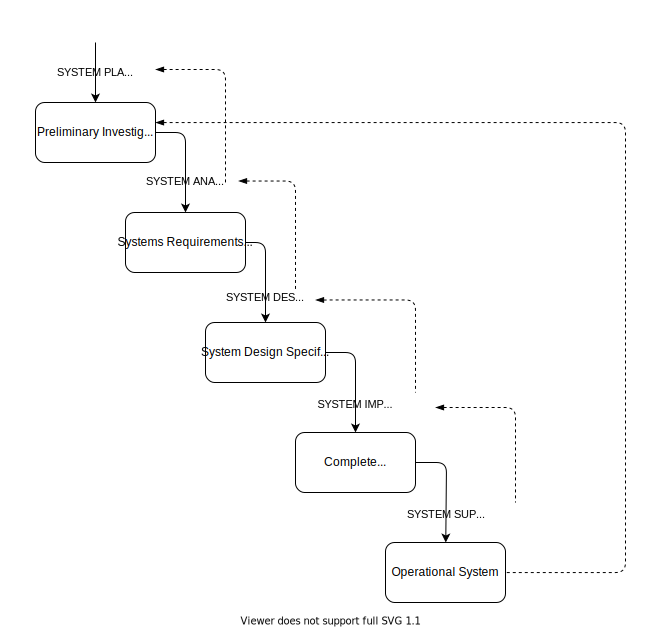
\includegraphics[width=350px]{Images/waterfall-v3.png}
    \caption{Waterfall Methodology Illustration showing the phases and deliverables for each phase}
    \label{waterfall-SDLC-method-image}
\end{figure}
\vspace{10px}


\subsubsection{System Planning}
\noindent Project planning is at the heart of the project life cycle, and tells everyone involved where you are going and how you are going to get there. This is where we shall document the project plan, define the project requirements and deliverables, and create the project schedule. It will involve creating a set of plans to help guide our team through the implementation and closure phases of the project. The plans created during this phase will help us manage time, cost, quality, changes, risk, and related issues. 

\subsubsection{Requirements Definition}
\noindent In this phase, all requirements of the project are defined and documented in a specification document and a feasibility analysis is done to check if these requirements are valid. At this stage, we shall gather data from the desired sample of the population about the different aspects of their diet and nutrition. The collection of this data will involve different steps that include; Identify issues and opportunities for collecting data, setting goals and objectives, planning approaches and methods, and collecting data. The collected data will enable us to answer stated research questions, test hypotheses, and evaluate outcomes.\\

\noindent In our research process, we shall use a hybrid method comprises of both qualitative and quantitative methods to carry out the data collection process. We shall use Makerere University as our case study specifically the students and because we are part of the community, collecting the information will be much easier.\\

\noindent Among the tools we shall use will include an online questionnaire which will be sent to students from colleges which will be grouped into two and the first group will be comprised of undergraduate students from colleges such as CHS, CEDAT and COCIS among others. This will be aimed at gathering information from continuing students, so that we can get a chain of events and know how their feeding has changed all over the years and benefits or set backs they have faced with meals while at the university.\\

\noindent We shall use the interviews and observation techniques to understand the patterns students use to select their daily meals at the different break intervals during the course of the day.\\

\subsubsection{System Analysis}
\noindent Also, at this stage, we will analyze how the system will meet user needs. The requirements gathered will be both functional and non-functional requirements. For example, Functional include “The system should authenticate a user’s new account in order to gain access.” Non-functional “The system should be able to handle 50 users without performance deterioration.” and others. After thorough analysis, a Requirements Understanding Document (RUD) is created.\\

\noindent The main purpose of conducting system analysis is to study the various processes and to find out its requirements. This includes methods of processing data and producing information. The determination of requirements entails studying the existing details about it to find out what these requirements are. The data will be analyzed with Google Form tools so that we can get matching patterns and also filter out what is necessary for us to be able to determine the users needs.\\

\noindent We will come up with a System requirements document that helps formalize the functional and non-functional requirements\\

\subsubsection{System Design}
\noindent At the design stage, we will describe the needs and behaviors that the system can perform in the form of UML. UML diagrams that we will make include; use Case diagram, class Diagram and activity diagram. We will also come up with wire-frames, mock-up designs for the user interface.\\

\noindent \textbf{Use Case Diagram for Web-based Application\\}
\noindent We shall visualize what actors can do with the system with each actor having different role(s), either student or an administrator.\\

 \textbf{Some of the actions that students will be able to perform are:}
\begin{enumerate}
\item Create a user account for access.
\item Enter their bio data while creating a user account.
\item Choose and select varieties of meal plans.
\item Give feedback and reviews on the quality of nutritional literature.
\item And Others.
\end{enumerate}

 \textbf{Some of the actions that an administrator will be able to perform are:}
\begin{enumerate}
\item Create or delete certain user accounts.
\item Update the number or meal plans available.
\item Increase or reduce the number of food groups available for the meal plans.
\item And Others.
\end{enumerate}

\noindent \textbf{Activity Diagram \\}
\noindent To start using this system, the user must first enter the system address. Users will be categorized into two, namely student and administrator. Students will have to register themselves in order to choose a meal plan via the web-based application. For an already registered student, they will have to login. If the username or password entered is incorrect,they will be denied access to the system and in case they forget it, the user can recover the password. After logging in the student can see monthly diet on the system dashboard for the respective user category.\\

\noindent \textbf{UML Class Diagram \\}
\noindent Each class has different responsibilities and functions commonly referred to as attributes and operations. Classes will include the following; User class which will be used in system authentications, with categories of administrator and student. Administrator and student classes will be used to in-cooperate the user’s bio-data. These are just a few of the classes that we will have.

\subsubsection{System Implementation}
\noindent The system will be implemented using programming languages and system implementation tools. While developing the database, we shall use MySQL which is an open-source language developed by Oracle.  \\

\noindent As a group, we will be utilizing a combination of different technologies to develop the front-end system. These include Hypertext Markup Language (HTML), Cascading Style Sheets (CSS), JavaScript, the Laravel framework and MySQL. Each of these technologies will play a specific role in the development process and will be used to create a dynamic, user-friendly and reliable web application. \\

\noindent \textbf{Hypertext Markup Language (HTML)\\}
\noindent We will use Hypertext Markup Language (HTML) for structuring and displaying the content on the web browser. It is the foundation of all web pages and is the standard markup language used to create web pages.\\

\noindent \textbf{Cascading Style Sheets (CSS)\\}
\noindent We will use Cascading Style Sheets (CSS) for enhancing the visual appearance of the web pages. It allows us to control the layout, colors, and fonts of web pages, making them more attractive and consistent.\\

\noindent \textbf{JavaScript\\}
\noindent We will use JavaScript for providing interactivity and dynamic functionality to the front-end. It allows us to create responsive and user-friendly features such as form validation and animations.\\

\noindent \textbf{Laravel Framework\\}
\noindent We will use the Laravel framework for managing and organizing the back-end functionality. It is a popular PHP framework that provides a simple and elegant syntax and is widely used for web application development.\\

\noindent \textbf{MySQL\\}
We will use MySQL for handling and managing data storage. It is a widely used and powerful relational database management system that is known for its reliability and performance. It will ensure that our application can handle any data size with great accuracy and efficiency.


\subsubsection{System Testing and Validation}
\noindent \textbf{System Testing \\}
\noindent The aim of testing a system is to ensure that a system meets its specification and any non-functional requirements (such as stability and throughput) that have been agreed upon with its users.\\

\noindent Each feature of the diet and nutrition management system, for example the BMI calculator, Timely Reminder, and Food Suggestions will be tested independently after being developed to see whether they function as intended.\\

\noindent System testing will be done while referring to the requirement specifications of the system to see if the developed system satisfies the predefined functionalities. The testing can be done through unit testing, integration testing, and user acceptance testing. \\

\noindent \textbf{Unit Testing \\}
\noindent This is where we shall identify individual functions that will be used in the system and this can involve testing a function that returns the number of meals stored in the system. To carry out unit testing, we will use a testing library/feature for the programming language in use. This process is majorly done to ensure that the functions are acting like they were intended. \\

\noindent \textbf{Integration Testing \\}
\noindent After all functions are working fine, we shall move on to integration testing where all the functions are put together and then testing if they all work to get the needed output.\\

\noindent \textbf{User Acceptance Testing \\}
\noindent This is the final type of testing and it is done by the end users to ensure that everything is working out fine and this will involve getting some students and allowing them to fully use the system for a specific number of days and then get feedback about the functionality of the system. 


%*******************************************************
%*******************************************************

\begin{table}[H]
\centering
\caption{Tabular Representation of the Methodologies}
\label{tab:representation-of-methodologies}
%--------------------------------
% Spacin Added By Victor
\setlength{\tabcolsep}{6pt}%sets the horizontal (column) spacing
\renewcommand{\arraystretch}{1} %sets the vertical (row) spacing
%--------------------------------
\resizebox{\columnwidth}{!}{%
\begin{tabular}{|l|l|l|l|}
\hline
\textbf{Objectives} & \textbf{Stage} & \textbf{Tool(s)} & \textbf{Output} \\ \hline
\begin{tabular}[c]{@{}l@{}} To identify \\requirements for \\the Diet \\Management system \end{tabular} & System Planning & Online Google Form & \begin{tabular}[c]{@{}l@{}} System Requirements \\Document \end{tabular} \\ \hline
\begin{tabular}[c]{@{}l@{}} To design a model \\for the system \end{tabular} & System Design  & \begin{tabular}[c]{@{}l@{}} Draw.io/Diagram.net\end{tabular} & \begin{tabular}[c]{@{}l@{}} System Design \\Document\end{tabular} \\ \hline
\begin{tabular}[c]{@{}l@{}} To implement the System\end{tabular} & \begin{tabular}[c]{@{}l@{}} System Implementation \end{tabular} & \begin{tabular}[c]{@{}l@{}} MySQL, HTML, \\JavaScript, CSS, PHP\end{tabular} & \begin{tabular}[c]{@{}l@{}} System for \\Testing\end{tabular}\\ \hline
\begin{tabular}[c]{@{}l@{}} To test and validate \\the System\end{tabular} & \begin{tabular}[c]{@{}l@{}} System Testing/Support and validation \end{tabular} & \begin{tabular}[c]{@{}l@{}} Software testing tools \\such as programming \\language testing \\libraries, visual Basic  \end{tabular} & \begin{tabular}[c]{@{}l@{}} Fully Developed \\System \end{tabular}\\ \hline

\end{tabular}%
}
\end{table}



%*******************************************************
%*******************************************************

\subsection{Conclusion}
\noindent This section fully states a detailed number of steps that will be followed to collect the data, process it and analyze it in order to get the specific requirements of the system which will then be used to design, develop, test and validate the system. \\

%%-------------------------------------------------------------------------------
%% xxx DOcument End xxx
%%-------------------------------------------------------------------------------
% \bibliographystyle{apa}% Set the bibliography style
% \bibliography{citation} % Include the bibliography file

%%-------------------------------------------------------------------------------
%% xxx Biblioraphy
%%-------------------------------------------------------------------------------
\newpage
\setlength\bibitemsep{3.0\itemsep}
\printbibliography


%%-------------------------------------------------------------------------------
%% xxx Appendix
%%-------------------------------------------------------------------------------
\newpage
\appendix
\renewcommand{\thesection}{} % Remove Numbering
\renewcommand{\thesubsection}{} % Remove Numbering
\section{Appendix A: Project Timeline}
\begin{tabular}{|l|l|l|}
\hline
\multicolumn{3}{|c|}{\begin{tabular}[c]{@{}l@{}} \\\textbf{Project part 1 completed} \vspace{20px} \end{tabular}} \\
\hline
\textbf{Activity} & \textbf{Duration} & \textbf{Deliverables} \\ \hline
Concept paper & 2 weeks & Problem statement and objectives \\ \hline
Literature review & 2 weeks & \begin{tabular}[c]{@{}l@{}} Overview of previously developed \\ systems relating to the topic \end{tabular} \\ \hline
Methodology & 2 weeks &  \begin{tabular}[c]{@{}l@{}} Summary of how the project objectives will\\ be achieved \end{tabular} \\ \hline
Proposal & 1 week & \begin{tabular}[c]{@{}l@{}} Summary of concept paper, literature \\review, and methodology  \end{tabular}   \\ \hline
\multicolumn{3}{|c|}{\begin{tabular}[c]{@{}l@{}} \\\textbf{Project part 2} \vspace{20px} \end{tabular}} \\
\hline
\textbf{Activity} & \textbf{Duration} & \textbf{Deliverables} \\ \hline
\begin{tabular}[c]{@{}l@{}} Data collection and deriving \\of system requirements  \end{tabular}& 3 weeks & System requirements document \\ \hline
\begin{tabular}[c]{@{}l@{}} Implementation, testing and \\ validation of the system  \end{tabular}& 8 weeks & Fully developed system \\ \hline
Conclusions and future work & 3 weeks & Final report \\ \hline
\begin{tabular}[c]{@{}l@{}} Developing slides \\for the developed system \end{tabular} & 1 week & Presentation \\ \hline
\end{tabular}

\newpage
\section{Appendix B: Project Budget}
\noindent As a group of students developing a diet and nutrition management system, we have considered the following budget to complete the project: \\

\begin{table}[h]
\caption{Estimated Budget}
\label{budget}
\begin{Large}
\begin{center}
\begin{tabular}{|l|r|}

\hline
\textbf{Item} & \textbf{Total cost (UGX)} \\ \hline
API costs for Nutrition data & 700,000 \\ \hline
Mobile Money integration costs & 800,000 \\ \hline
Research costs & 600,000 \\ \hline
Equipment costs & 200,000 \\ \hline
Printing and stationary costs & 100,000 \\ \hline
Miscellaneous (e.g. Transport, Lunch,etc) & 600,000 \\ \hline
\textbf{Total} & \textbf{3,000,000} \\ \hline
\end{tabular}
\end{center}
\end{Large}
\end{table}
\vspace{10pt}
\textbf{Note:} The above budget is a rough estimate, and the actual costs may vary depending on the specific requirements and scope of the project. Also, this budget is purely an estimate and it might change based on the need of the project. However, it is worth noting that this budget will only cover the costs of items such as API subscriptions, mobile money integration, research, equipment, printing and stationary, and miscellaneous expenses for the group of 5 students. The development costs are not included as it is assumed that we will be developing the system ourselves. This can be used as a guide for us to develop a diet and nutrition management system for students at Makerere University.


\newpage
\section{Appendix C: A guide to data collection using questionnaires and interviews}

\noindent We are third-year students at the College of Computing and Information Technology (COCIS) and we are developing a diet and nutrition management system that will help students manage their diets effectively. The system will allow students to register and based on their input, the system will provide timely reminders, food suggestions, and nutrition literature. This is an endeavor to help a student improve their overall mental health, especially regarding memory retention and the intelligence quotient.\\

\subsection{Sample questions for the questionnaire guide directed to Makerere University students}
\begin{enumerate}
\item What is your name?
\item What is your gender?
\item When did you join Makerere University?
\item Which college are you from?
\item Do you cook your meals or do you have them from a restaurant?
\item What is the average price of the food you eat?
\item If you have your meals from out, where do you go?
\item Do you have a clear time frame for your meals?
\item Do you have a consistent meal plan?
\item How many meals do you have in a day?
\item Are these the same number of meals that you have been consuming since you joined the university?
\item If no, why?
\end{enumerate}

\subsection{Interview Guide for Makerere Students}
\begin{enumerate}
\item What is your name?
\item When did you join Makerere University?
\item Which college are you from?
\item Do you cook your meals or do you have them from a restaurant?
\item What is the average price of the food you eat?
\item If you have your meals from out, where do you go?
\item Do you have a clear time frame for your meals?
\item Do you have a consistent meal plan?
\item How many meals do you have in a day?
\item Are these the same number of meals that you have been consuming since you joined the university?
\item If no, why?
\end{enumerate}

\subsection{Interview Guide for Doctors}
\begin{enumerate}
\item What is your name?
\item What are the general effects of not having a balanced diet?
\item What impact does an improper diet have on a student’s mental health and concentration?
\item What is the most suitable time for students to have their meals?
\item What are the best food combinations that will help a student achieve a balanced diet?
\item What calories are contained in certain foods and how much should be consumed?
\item What do you consider as over and under-eating?
\item How could we access your nutritional literature?
\item What advice do you have for students concerning their diet?
\end{enumerate}


\end{document}
